\documentclass[Main]{subfiles}

\begin{document}


\chapter{Indledning}

\begin{figure}[H]
\centering
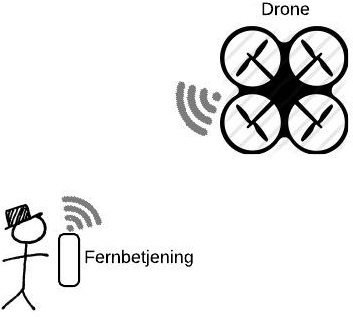
\includegraphics[width = 0.40 \textwidth]{System}
\caption{Systemoversigt}
\label{Fig:System}
\end{figure}
På figur \ref{Fig:System} ses et oversigt over det samlede system. Opgaven var at lave lavfrekvent styring af en drone.Systemet skulle bestå af en fjernbetjening og en drone af mærket AeroQuad. Målet var at kunne styre dronen med en fjernbetjening, ved en frekvens på 433MHz. Derudover skulle dronen også være i stand til at holde sin højde. Dronen skulle også selv kunne undgå at flyve ind i objekter foran den, selvom brugeren beder den om det.

Systemet består af:
\begin{enumerate}
\item AeroQuad Drone
\item Trådløs fjernbetjening
\end{enumerate}














\end{document}